\section{Methoden}
\subsection{Zeitmaße}

Es existieren verschiedene Zeitmaße mit unterschiedlichen Definitionen, die im folgenden aufgeführt sind.
\begin{itemize}
\item Wahre Sonnenzeit (WZ): Die wahre Sonnenzeit wird am Stand der Sonne am Himmel gemessen und beträgt 12 Uhr, wenn die Sonne durch den Meridian des Standortes geht.
\item Mittlere Sonnenzeit (MZ): Die mittlere Sonnenzeit ist eine kurzfristig gleichmäßig vergehende Zeit, wobei eine fiktive mittlere Sonne den Zeitverlauf bestimmt. Sie läuft längs des Äquators
\item Weltzeit, Universal Time (UT): Die Weltzeit ist ein Zeitmaß, das aufgrund internationaler Vereinbarungen für jeden Ort die gleiche Zeit liefert. Sie entspricht dabei der mittleren Sonnenzeit auf dem 0-Meridian.
\item Zonenzeit: Als Zonenzeit wird eine einheitliche Zeit innerhalb einer Zeitzone bezeichnet. Dabei wird die Erde in 24 Zeitzonen eingeteilt, um innerhalb einer Zeitzone vertretbare Abweichungen von der mittleren Sonnenzeit zu gewährleisten.
\item Julianisches Datum (JD): Das Julianische Datum gibt die Tage an, die seit dem 1. Januar -4712, 12 Uhr vergangen sind.
\item Sternzeit, Sidereal Time (ST): Die Sternzeit ist ein Zeitmaß, das auf der scheinbaren Rotation der Sterne am Himmel, hervorgerufen durch die Erdrotation, beruht. Ein Sterntag ist die Dauer, die der Sternenhimmel für ein ganze scheinbare Umdrehung benötigt. Die ST definiert sich als Stundenwinkel des Frühlingspunkts.
\item Ephemeridenzeit (ET,TT oder TDT): Die Ephemeridenzeit ist ein durch die Dynamik des Sonnensystems definiertes Zeitmaß. Eine Ephemeridensekunde entspricht dabei dem 31.556.925,9747ten Teil des Tropischen Jahres 1900. 
\item Atomzeit: Die Atomzeit ist ein Zeitmaß das auf der SI-Sekunde basiert und wird weltweit bei zahlreichen Zeitinstituten in der Regel durch Cäsium-Atomuhren realisiert. Eine Sekunde ist das 9.192.631.770-fache der Periodendauer der dem Übergang zwischen den beiden Hyperfeinstrukturniveaus des Grundzustandes von Atomen des Nuklids Cs-133 entsprechenden Strahlung.
\end{itemize}

Dabei verlaufen die Ephemeridenzeit und die Atomzeit streng gleichförmig, ungleichmäßig dagegen verlaufen die mittlere Sonnenzeit, die Weltzeit und die Zonenzeit aufgrund der Schwankungen der Erdrotation.

Die wahre Sonnenzeit verläuft aus zwei Gründen ungleichmäßig: Zum einen wird der gleichmäßige Verlauf durch die elliptische Form der Erdbahn und zum anderen durch die Neigung der Erdachse gestört.

Die Sternzeit steht unter dem Einfluss von Schwankungen der Rotation der Erde, wie z.B. die Präzession. Daher verläuft die Sternzeit nicht streng gleichförmig.

\subsection{Astronomische Koordinatensysteme}
Für diese Messung sind drei Koordinatensysteme von besonderer Bedeutung.

\subsubsection{Horizontsystem}

Der Ursprung des Horizontsystems liegt beim Beobachter, der Grundkreis ist der lokale Horizont. Längen- und Breitenkoordinaten entsprechen Höhenwinkel und Azimut. Die Pole sind Zenit und Nadir, wesentlicher Verwendungszweck sind Messungen an der Erdoberfläche. 

\subsubsection{Festes Äquatorsystem}

Beim festen Äquatorialsystem liegt der Ursprung wahlweise im Beobachter oder im Erdmittelpunkt. Der Grundgkreis ist hier der Himmeläquator, Längen- und Breitengrad entsprechen Deklinations- und Stundenwinkel. Die Pole sind die Himmelspole selbst. Verwendet wird dieses System vor allem bei astronomischen Beobachtungen. 

\subsubsection{Bewegliches Äquatorsystem}

Das bewegliche Äquatorialsystem entspricht dem festen, bis auf den Unterschied, dass Längen- und Breitengrad Deklinationswinkel und Rektazension entspricht. 

\subsection{Azimut und Höhe}
In einem Koordinatensystem mit einer Grundebene, welche im Fall etwa des Horizontsystems die Erdoberfläche ist, und einem dazu senkrechten Zenit, definiert man die Deklination als den Winkel zwischen Objekt und der Grundebene, sowie den Azimut als Winkel relativ zu einer ausgezeichneten Richtung. Im Fall des Horizontsystems ist dies etwa die Nord-Süd-Richtung, wobei 0 $^\circ$ Süden entspricht und die Zählung über Westen, Norden und Osten fortgesetzt wird.  

\subsection{Der Theodolit}
Für die Bestimmung der relativen Azimutwerte wird ein Theodolit verwendet, welcher mittels einer Montierung auf den Teleskopsäulen im Garten befestigt werden kann. Ein Bild des Theodoliten ist Abbildung \ref{fig:Theodolit}, welche auf Seite \pageref{fig:Theodolit} zu finden ist. An der Montierung wird ein Element in Form eines regelmäßigen Dreiecks befestigt, das mittels zweier Feinhorizontierschrauben relativ zur Montierung bewegt werden kann, allerdings nur um sehr kleine Wege. Dieser Mechanismus dient der Feineinstellung. Der Rest des Theodoliten ist mit einem Kugelgelenk mit dem vorherigen Element verbunden. \\
Daran schließt sich der eigentliche Theodolit an: Dieser ist zum einen drehbar um die vertikale Achse, zum anderen drehbar um eine horizontale Achse gelagert, sodass nun jeder beliebige Punkt am Himmel durch das sich anschließende Fernrohr anvisiert werden kann.  Des weiteren existiert eine Einrichtung zur Einstellung des Nullpunktes der Azimut-Skala sowie eine Wasserwaage, mit der die horizontale Ausrichtung des Theodoliten geschieht. \\
Im ersten Schritt soll der Theodolit horizontal ausgerichtet werden, sodass sich also bei einer Drehung des Theodoliten um die vertikale Achse nur der Azimut des betrachteten Objekts ändert und nicht dessen Deklination.\\
Dazu wird zunächst der Theodolit mittels des Kugelgelenks und einer Libelle (kreisförmige \enquote{Wasserwaage}) grob horizontal ausgerichtet. Die Feinjustierung geschieht dann mittels eines Algorithmus, mit dem man sich der horizontalen Ausrichtung annähert: Zunächst wird die Wasserwaage entlang einer Seite der dreieckigen Grundfläche ausgerichtet und die Ausrichtung des Theodoliten mit der entsprechenden Feinhorizontierschraube exakt auf Null eingestellt. Danach wird der Theodolit um 180 $^\circ$ um die vertikale Achse gedreht und der neue Ausschlag der Luftblase mittels der gleichen Feinjustierschraube halbiert. Anschließend wird der Theodolit um selbige Achse nochmals um 90 $^\circ$ gedreht und der Ausschlag der Luftblase mit der zweiten Feinhorizontierschraube auf den vorherigen Spielpunkt eingestellt. Indem dieses Vorgehen wiederholt wird, erreicht man nach ausreichend vielen Wiederholungen eine hinreichend genaue horizontale Justierung des Theodoliten. \\

\begin{figure}
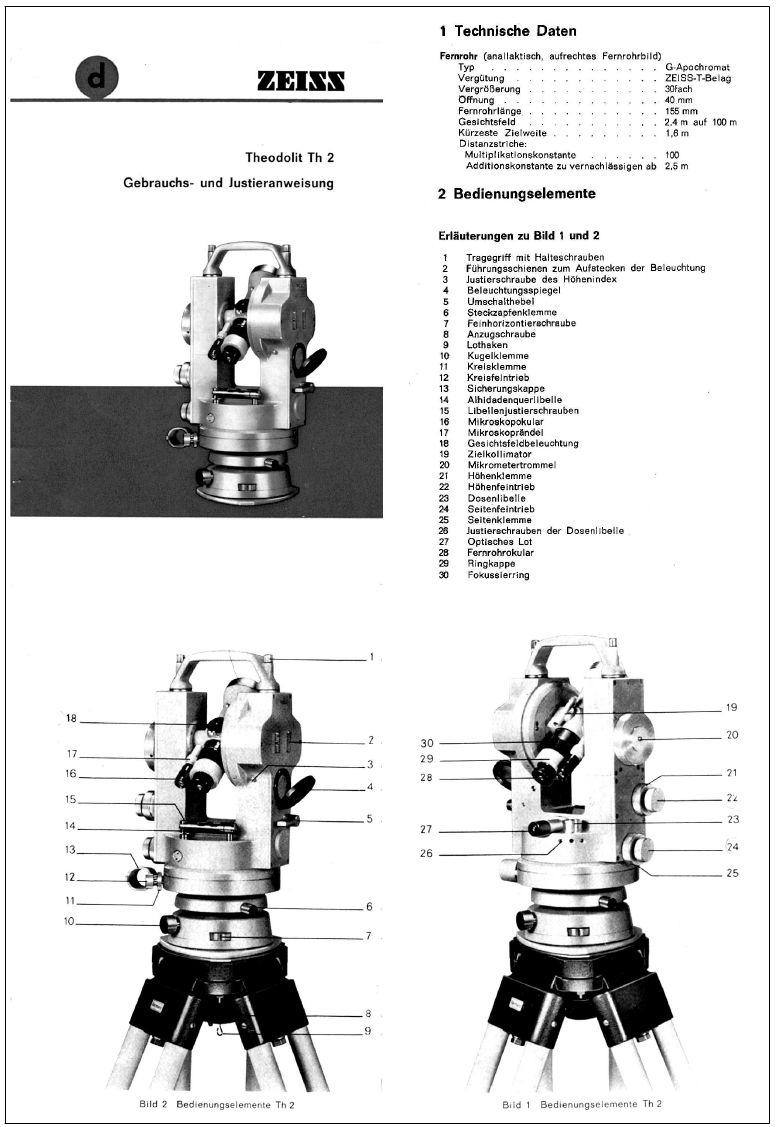
\includegraphics[width=1\textwidth]{images/theodolit}
\caption{Bild des Theodoliten mit Kennzeichnung der einzelnen Teile}
\label{fig:Theodolit}
\end{figure}

\subsection{Messungen mit dem Theodoliten}
Azimut und Deklination eines Objekts können bestimmt werden, indem das entsprechende Objekt anvisiert wird. Durch Umlegen eines Schalters kann man zwischen Höhe und Azimut wechseln. Der entsprechende Wert kann dann durch das Mikroskoprändel angelesen werden. Dazu muss die Mikrometertrommel derart eingestellt werden, dass die Lücken in den beiden sichtbaren Balken exakt nebeneinander liegen. 

\subsection{Messung des Turmazimuts}
Mit einem derart justierten Theodoliten können nun Azimut und Höhe eines Objekts am Himmel bestimmt werden, indem man das entsprechende Objekt anvisiert und auf der Skala nun den jeweiligen Winkel, der in gon angezeigt wird, abliest. Dabei kann die Höhe als absoluter Wert im Horizontsystem abgelesen werden, wohingegen der Azimut nur relativ zu einem frei einstellbaren Nullpunkt bestimmbar ist. \\
Um nun den Azimut des angesprochenen Objekts zu bestimmen, wird nun der relative Azimut des Objekts sowie der Azimut eines anderen Objekts abgelesen, der beispielsweise mittels Literatur- und Tabellenwerten als absoluter Wert bestimmt werden kann. Dieses zweite Objekt ist in diesem Fall die Sonne. \\
Um den Turmazimut zu bestimmen, wird das Objekt mittels des Fadenkreuzes derart anvisiert, dass sich die Turmspitze möglichst exakt zentral im Fadenkreuz befindet. \\

\subsection{Messung des Sonnenazimuts}
Da die Sonne nicht direkt durch das Fernrohr beobachtet werden kann, da dies zu einer sofortigen Schädigung des Auges und der Sehfähigkeit führen würde, muss hierfür ein Filter verwendet werden. Bei der Messung wurden eine Kombination aus einem UV-IR-Rejection-Filter sowie aus zwei Neutraldichte-Filtern mit den Werten 1.8 und 3.0 eingesetzt. \\ 
Zur Bestimmung des Sonnenazimuts wird ein Überstreichen der Sonnenscheibe über einen senkrechten Strich des Fadenkreuzes betrachtet. Mit einer Stoppuhr wird eine Zeitmessung gestartet, wenn der rechte Rand der Sonnenscheibe jenen Strich berührt. Wenn der linke Rand den gleichen Strich überstreicht, wird eine Zwischenzeit genommen, zu einem frei gewählten Zeitpunkt, der ebenfalls notiert wird, wird schließlich die Messung beendet. Aus diesen drei Messungen kann der Zeitpunkt in MEZ bestimmt werden, an dem das Zentrum der Sonnenscheibe das Zentrum des Fadenkreuzes überstreicht. Der Zeitpunkt, zu dem das Zentrum der Sonne das Zentrum des Fadenkreuz überstreicht, kann einfach mittels der folgenden Formel bestimmt werden: 
\begin{equation}
U_{zen} = U_{end} - (t_{end} - \frac {t_{zw}}{2}), 
\end{equation}
wobei $U_{zen}$ die Uhrzeit des Zentrumdurchgangs, $U_{end}$ die Uhrzeit bei Beendigung der Messung, $t_{end}$ die von der Stoppuhr am Ende der Messung angezeigte Zeit sowie $t_{zw}$ die gemessene Zwischenzeit auf der Stoppuhr. 

\subsection{Berechnung des absoluten Sonnenazimuts}
Mittels der in Listing \ref{script} (Anhang) dargestellen Berechnung kann aus Tabellenwerten für die Sternzeit um 0 Uhr des Messtages in Greenwich, den aktuellen Offset zwischen universal time (UT) und Ephemeridenzeit (TT) sowie den Werten für die Sonnendeklination und die Rektaszension im Äquatorialsystem zu Beginn und Ende des Messtages der absolute Azimut der Sonne zu jedem Messzeitpunkt eines Wertes für den Sonnenazimut bestimmt werden. Daraus ergibt sich durch Mittelung der Offset zwischen dem eingestellten Nullpunkt des Azimuts und der Nord-Süd-Verbindung. 
Durch Addition des Unterschiedes zwischen den relativen Azimutwerten für Turm und Sonne kann so der absolute Azimut des Turms bestimmt werden. 